\chapter{Evaluation}
\label{s:eval}

\paragraph{Evaluation Goals} We evaluated our work on security and performance. We want our work to
meet the conditions established in \autoref{d:isolation}, and we want performance overhead to be
within acceptable levels. When we designed our approach, our target for performance was a negligible
slowdown within both memory-safe code and memory-unsafe code, with only a small performance penalty
when entering or exiting a sandboxed function.

\section{Security}

Recall our security definition in \autoref{d:isolation}. In order for our sandboxing scheme to be
considered secure, the sandboxed portion of the program must not allow sandboxed code to write to
memory allocated within safe code, and it must prevent memory corruption that occurs within
sandboxed code from causing undefined behavior within safe code.

We use MPK to enforce our first condition ("Memory allocated within safe code cannot be written by
sandboxed code"). In particular, we achieve this by our configuration of the PKRU register to deny
write access to protected data upon entering sandboxed code, and to re-enable write access upon
exiting sandboxed code. More specifically, we assume the processor's implementation of MPK is itself
correct and secure (in other words, that an attacker truly cannot write to memory restricted by
MPK).

We also must ensure that an attacker with partial or complete control over the program's execution
cannot cause a \cc{wrpkru} instruction to be executed and maintain control of the program
afterwards, as this would potentially allow an attacker to disable the sandboxing restrictions and
corrupt protected memory. We enforce this by ensuring the return address and call stack used by safe
code are not writable by sandboxed code, preventing the attacker from using a backward-edge control
flow hijacking attack to redirect code execution after the program returns from the sandbox to safe
code. Additionally, we require that the program does not use the \cc{wrpkru} instruction except for
entering and exiting the sandbox, and we require the use of Control-flow Enforcement Technology
(CET) to prevent the attacker from using a forward- or backward-edge control flow hijacking attack
(such as function pointer hijacking or return-oriented programming) to cause the execution of a
\cc{wrpkru} instruction.

The second condition is more difficult to verify, as in general, it is impossible to reason about a
program in the presence of undefined behavior such as memory corruption. In theory, the compiler
could identify undefined behavior in the sandboxed code and as a result generate \cc{wrpkru}
instructions that defeat our sandboxing; generate unexpected code within the safe portions of our
program that assume the sandboxed portions do not induce undefined behavior; trigger unknown
processor bugs that defeat MPK, or ``make demons fly out of your nose'' (as the saying goes).
However, in order to reason about systems security, we must make assumptions constraining undefined
behavior to reasonable limits. Since an attacker can and will exploit undefined behavior to attack a
system, we must design our systems to maintain their security model in the presence of undefined
behavior, and we must rely on the layers below us to uphold the security guarantees we rely on. For
instance, operating systems must assume that a processor's memory protection guarantees apply even
in the presence of a program inducing undefined behavior; system call interfaces must uphold their
security models even when provided with invalid or impossible inputs; and in-process sandboxing
schemes like ours must assume the compiler does not introduce optimizations that violate our
sandboxing requirements even in the presence of undefined behavior. In practice, this assumption may
not always hold; designing systems that are correct in the face of unexpected compiler behavior is a
limitation of any in-process sandboxing scheme and an area of active research.

Proceeding under the assumption that undefined behavior within the sandbox does not somehow disable
the sandbox, then to verify the second condition we only need to consider how the safe portions of
our program react upon receiving untrusted outputs from the sandbox. The Rust language guarantees no
undefined behavior, as long as the safe portions of our program do not incorrectly use \cc{unsafe}
language features, and as long as any \cc{unsafe} blocks do not return invalid values to the safe
portions of the program. Our \cc{bindgen}-generated interface contains \cc{unsafe} blocks for
integrating with unsafe code, but we believe all our \cc{unsafe} code to be correctly written and
free of undefined behavior. Our requirement that types exchanged across sandbox boundaries conform
to \cc{bytemuck::AnyBitPattern} means that unsafe code cannot produce invalid values (as no such
invalid values exist), and our bounds, alignment, and aliasing checks on pointers exchanged across
sandboxed boundaries ensures that invalid pointers cannot cause undefined behavior.

There may be a risk of induced undefined behavior through application binary interface (ABI)
violations. For instance, calling conventions typically specify a set of registers that are expected
to be preserved across function calls; most x86 calling conventions require that the direction flag
be clear when calling and returning from functions; and the ARM procedure call standard requires
that signed types shorter than 32 bits be sign extended when passed in registers. In theory, a
sandboxed application may induce undefined behavior in the safe portions of the program by violating
these ABI constraints; while our proof-of-concept is potentially vulnerable to this attack vector,
our work can be extended to defend against this possible attack by modifying the sandbox thunk
function to carefully verify ABI invariants upon exiting sandboxed code.

\section{Performance}

Our implementation only affects code generation when memory-safe code calls and returns from a
function defined in a sandboxed library. The sandboxed library remains unchanged, as does most of
the Rust application (aside from potential application-specific needs to copy data into or out of
sandboxed memory). Thus, we expect the performance impact of our work to manifest as a fixed
overhead per function call into a sandboxed library. Applications that interact with sandbox
libraries frequently via many short-lived function calls are expected to suffer the greatest
performance overhead, whereas we expect the performance impact to be negligible for applications
that make few or longer-running function calls.

To test this, we used the \cc{cargo bench} tool available in nightly Rust \cite{rust:cargo-bench}.
We created a series of three benchmarks: a microbenchmark which calls a sandboxed no-operation
function (to measure the overhead of a single function call), a second test case which uses the
\cc{cmark} Markdown parsing library \cite{cmark} to render a short string of Markdown into HTML, and
a third which uses \cc{cmark} to render a long document (created by concatenating all localizations
of the first edition of Pro Git \cite{pro-git}, as this is the document used by the authors of cmark
in their own benchmarks \cite{cmark:benchmarks}). \cc{cargo bench} automatically runs a sufficient
number of iterations of each benchmark to ensure statistically significant results, with the
iteration count determined dynamically based on the runtime of each tests and the level of noise in
the results. The \cc{nop} and \cc{cmark\_simple} microbenchmark results reported are an average over
several million iterations, and the \cc{cmark\_large} benchmark is an average over several hundred
iterations. We ran our benchmarks on an Intel NUC with an i5-1135G7 CPU running at 2.4 GHz.

We ran each test case under three conditions: once with sandboxing and control-flow enforcement
disabled to establish a baseline; once with sandboxing disabled but CET enabled so that we can
determine how much performance impact is caused by our sandbox and how much is caused by CET; and a
third time with sandboxing and CET enabled. The results are available in \autoref{bench-txt},
\autoref{f:graph1}, and \autoref{f:graph2}. \cc{cargo bench} is designed for accurate
microbenchmarking and runs each test case a sufficient number of iterations to obtain statistically
meaningful results.

\begin{figure}[ht]

\begin{subfigure}{1\textwidth}
\input{code/bench-nocet.txt}
\coderule
\caption{Sandboxing and CET disabled}
\end{subfigure}

\begin{subfigure}{1\textwidth}
\input{code/bench-nompk.txt}
\coderule
\caption{Sandboxing disabled, CET enabled}
\end{subfigure}

\begin{subfigure}{1\textwidth}
\input{code/bench-mpk.txt}
\coderule
\caption{Sandboxing and CET enabled}
\end{subfigure}

\caption{Benchmark results}
\label{bench-txt}
\end{figure}

\begin{figure}[ht]
    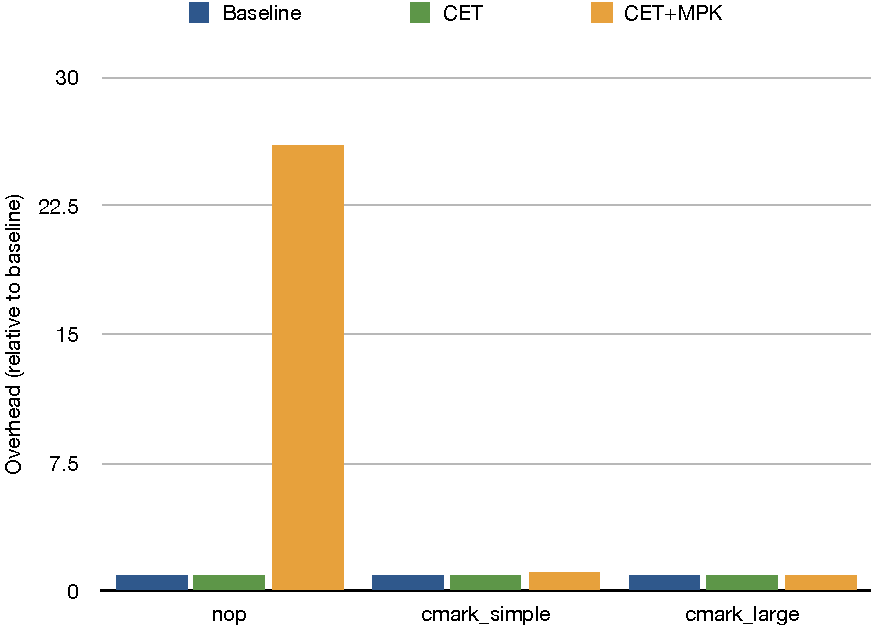
\includegraphics[width=\textwidth]{fig/graph1}
    \caption{Graph of benchmark results.}
    \label{f:graph1}
\end{figure}

\begin{figure}[ht]
    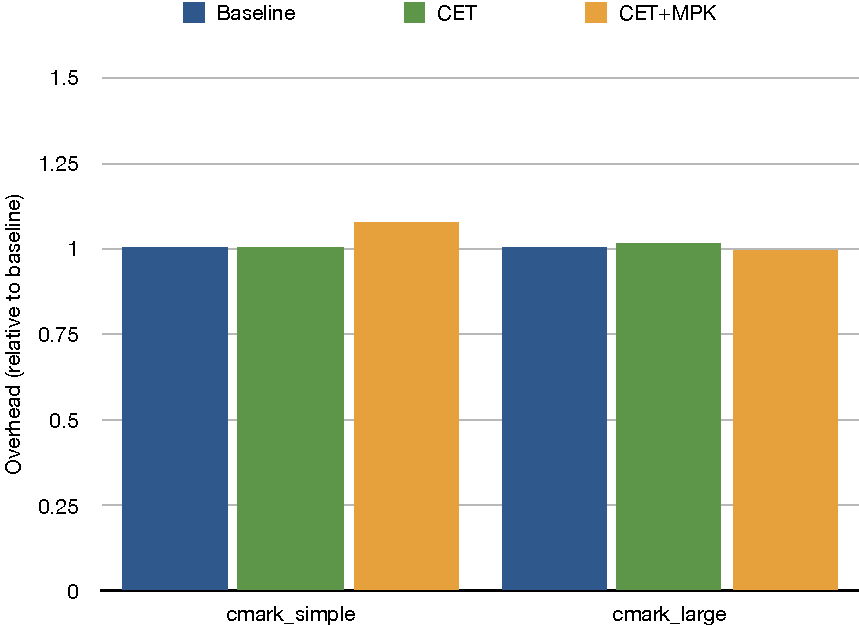
\includegraphics[width=\textwidth]{fig/graph2}
    \caption{Graph of benchmark results, excluding the \cc{nop} benchmark.}
    \label{f:graph2}
\end{figure}

The no-operation benchmark shows an overhead of approximately 25 nanoseconds due to our sandbox for
a single function call, compared to a baseline of 1ns. The small cmark benchmark runs approximately
50 nanoseconds slower when sandboxing is enabled, an overhead of about 7\%; this is consistent with
the no-op test case as the small cmark test case makes two sandboxed function calls. For the
longer-running cmark test case, the performance impact is not statistically significant (as the work
required to enter and exit the sandbox is dwarfed by the work performed within the sandbox.) The
benchmark results show no statistically significant performance impact caused by the use of CET. 
